% --------------------------------------------------------------
% This is all preamble stuff that you don't have to worry about.
% Head down to where it says "Start here"
% --------------------------------------------------------------

\documentclass[12pt]{article}

\usepackage[margin=1in]{geometry}
\usepackage{amsmath,amsthm,amssymb}
\usepackage{enumerate}
\usepackage{graphicx}
\usepackage[english]{babel}
\usepackage[utf8x]{inputenc}
\usepackage[T1]{fontenc}
\usepackage{enumitem}
\usepackage{fancyhdr}
\usepackage{MnSymbol,wasysym}
\pagestyle{fancy}
\usepackage{multirow}

\newcommand{\N}{\mathbb{N}}
\newcommand{\Z}{\mathbb{Z}}
\newcommand{\R}{\mathbb{R}}
\newcommand{\Q}{\mathbb{Q}}
\newcommand{\C}{\mathbb{C}}

\newenvironment{theorem}[2][Theorem]{\begin{trivlist}
\item[\hskip \labelsep {\bfseries #1}\hskip \labelsep {\bfseries #2.}]}{\end{trivlist}}
\newenvironment{lemma}[2][Lemma]{\begin{trivlist}
\item[\hskip \labelsep {\bfseries #1}\hskip \labelsep {\bfseries #2.}]}{\end{trivlist}}
\newenvironment{exercise}[2][Exercise]{\begin{trivlist}
\item[\hskip \labelsep {\bfseries #1}\hskip \labelsep {\bfseries #2.}]}{\end{trivlist}}
\newenvironment{problem}[2][Problem]{\begin{trivlist}
\item[\hskip \labelsep {\bfseries #1}\hskip \labelsep {\bfseries #2.}]}{\end{trivlist}}
\newenvironment{question}[2][Question]{\begin{trivlist}
\item[\hskip \labelsep {\bfseries #1}\hskip \labelsep {\bfseries #2.}]}{\end{trivlist}}
\newenvironment{corollary}[2][Corollary]{\begin{trivlist}
\item[\hskip \labelsep {\bfseries #1}\hskip \labelsep {\bfseries #2.}]}{\end{trivlist}}

\lhead{Assignment 3, April 9, 2022}
\rhead{Nicholas Tee}

\begin{document}

\section{RNN}
The hyper parameters that I used were the same as the recommended ones in the assignment file, except the drop-out rate which I did not include in my model.
\begin{table}[!h]
\centering
\begin{tabular}{|l|ll|l|ll|}
\hline
         & \multicolumn{2}{l|}{RNN}               &  & \multicolumn{2}{l|}{LSTM}            \\ \hline
Dataset  & \multicolumn{1}{l|}{train}   & test    &  & \multicolumn{1}{l|}{train}  & test   \\ \hline
Accuracy & \multicolumn{1}{l|}{99.12\%} & 60.12\% &  & \multicolumn{1}{l|}{99.5\%} & 70.1\% \\ \hline
\end{tabular}
\end{table}
The table above shows my results, its clear that the 20 epochs might have over fitted the model a little too much resulting in relatively low accuracies on the test sets.
\section{Proof}
\begin{figure}[h!]
	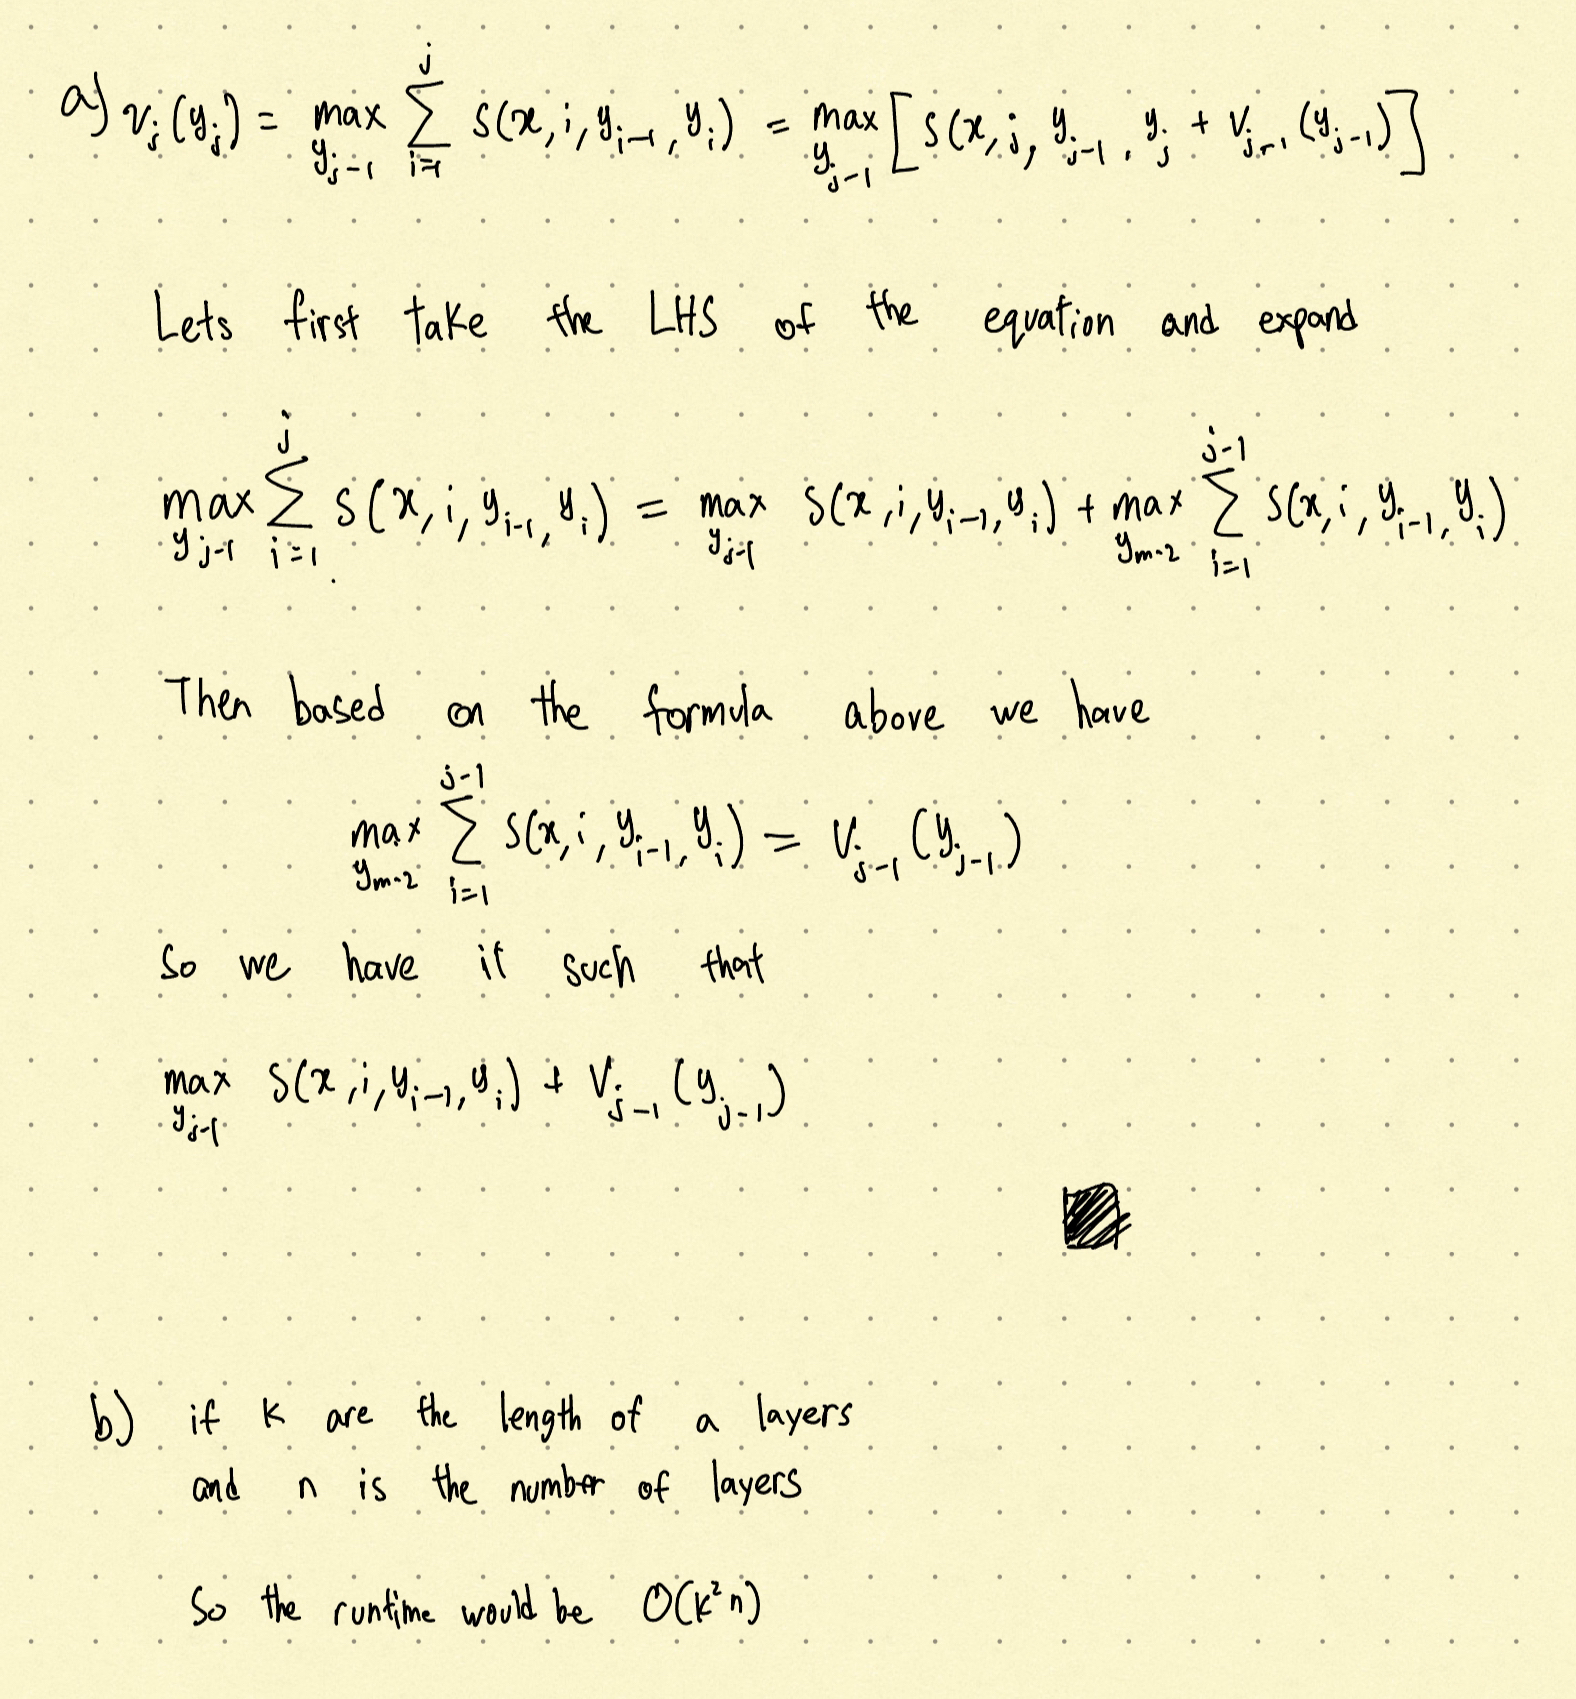
\includegraphics[scale=0.2]{2.png}
\end{figure}
\newpage
\section{Viterbi}
I wasn't sure which set of numbers we had to report, but these were the highest accuracies that I could attain. The top half of the numbers are the results from the \textbf{ner.test} and the bottom half are the numbers from the\textbf{ner.dev}
\begin{figure}[h!]
	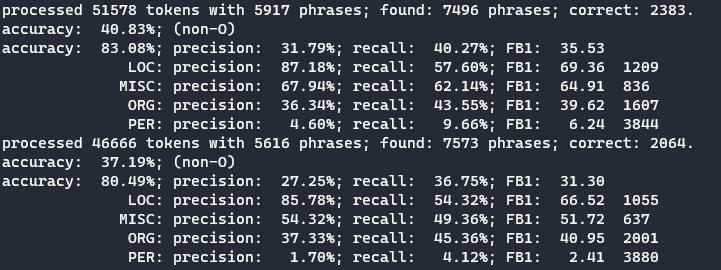
\includegraphics[scale=0.8]{1.png}
\end{figure} 
\end{document}















